\Exercise[number={5}]
A doctor measures the value of a parameter \(P\) to monitor the evolution
of a patient's disease.\\
Parameter \(P\) can assume the values \(\{low, high\}\). The value of \(P\)
is the effect of a state or condition \(C\), not directly observable,
which can be \(\{good, bad\}\).
The status changes from one day to the next in \(1/5\) of cases. If the
patient is in a \(good\) condition, the \(P\) value is \(low\) on \(8/10\)
samples. If the patient is in as \(bad\) condition, the \(P\) value is
\(high\) on \(7/10\) samples. Upon arrival at the hospital (day 0), the
patient's condition is unknown, i.e. \(Pr(C=good)=0.5\).
\begin{itemize}
    \item\quad a. Formulate a model of the problem and draw the
    corresponding temporal model, specifying the corresponding probability
    table for each node.
    \item\quad b. Calculate the probability that the patient is in a
    \(good\) condition on day 2, given that \(P\) had a \(low\) value on
    day 1 and \(high\) on day 2.
\end{itemize}

\Answer[number={5}]
a. Here there is a schematization for the model:
\begin{figure}[H]
    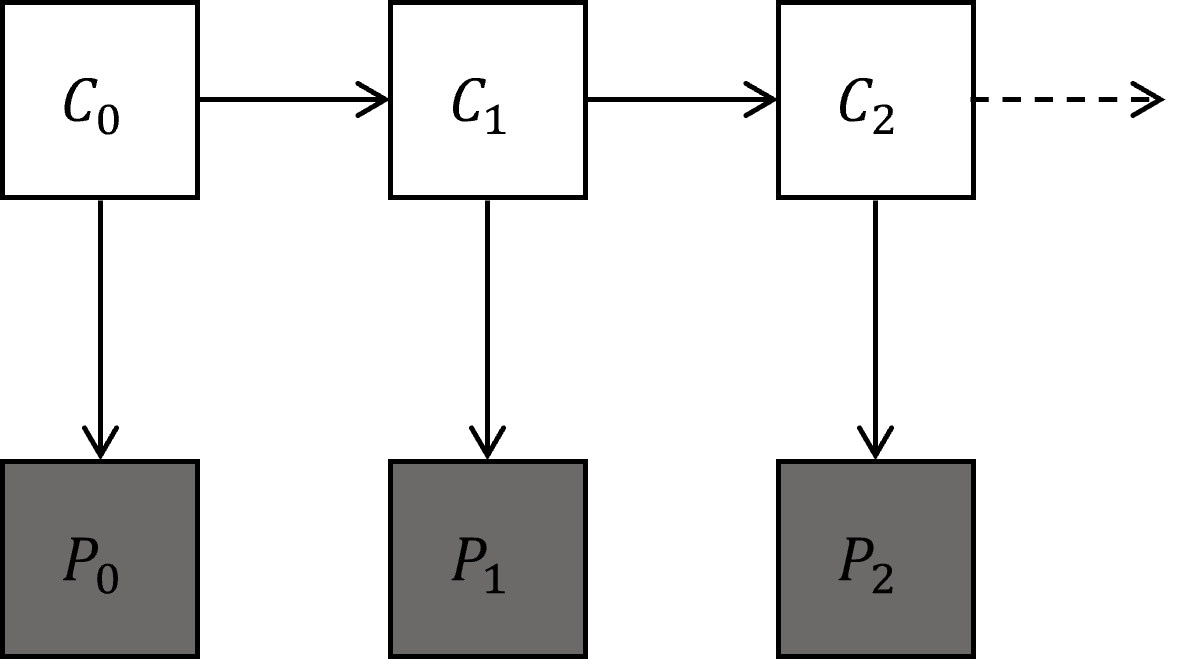
\includegraphics[scale=0.75]{E_5}
    \centering
\end{figure}
First of all, let's compute explicitly all the necessary probabilities:
\begin{align*}
    \begin{matrix}
        Pr(C_0=good)=0.5 && \Rightarrow && Pr(C_0=bad)=1-0.5=0.5\\
        Pr(C_{t}=good|C_{t-1}=bad)=0.2 && \Rightarrow && Pr(C_{t}=bad|C_{t-1}=bad)=1-0.2=0.8\\
        Pr(C_{t}=bad|C_{t-1}=good)=0.2 && \Rightarrow && Pr(C_{t}=good|C_{t-1}=good)=1-0.2=0.8\\
        Pr(P_{t}=low|C_{t}=good)=0.8 && \Rightarrow && Pr(P_{t}=high|C_{t}=good)=1-0.8=0.2\\
        Pr(P_{t}=high|C_{t}=bad)=0.7 && \Rightarrow && Pr(P_{t}=low|C_{t}=bad)=1-0.7=0.3
    \end{matrix}
\end{align*}
Then, the probability tables are:
\begin{align*}
    \begin{matrix}
        {} && C_0=good && C_0=bad\\
        Pr(C_0) && 0.5 && 0.5
    \end{matrix}
\end{align*}
\begin{align*}
    \begin{matrix}
        {} && C_t=good && C_t=bad\\
        Pr(C_t|C_{t-1}=good) && 0.8 && 0.2\\
        Pr(C_t|C_{t-1}=bad) && 0.2 && 0.8
    \end{matrix}
\end{align*}
\begin{align*}
    \begin{matrix}
        {} && P_t=low && P_t=high\\
        Pr(P_t|C_{t}=good) && 0.8 && 0.2\\
        Pr(P_t|C_{t}=bad) && 0.3 && 0.7
    \end{matrix}
\end{align*}
b. The probability that the patient is in a \(good\) condition on day 2,
given that \(P\) had a \(low\) value on day 1 and \(high\) on day 2 is:
\begin{align*}
    Pr(C_2=good|P_1=low,P_2=high)
    =Pr(C_2=good|C_0,C_1,P_0,P_1=low,P_2=high)
\end{align*}
In order to proceed, this conditional probability requires to be transformed
into a joint probability:
\begin{align*}
    Pr(C_2=good|P_1=low,P_2=high)
    =\frac{Pr(C_2=good,P_1=low,P_2=high)}{Pr(P_1=low,P_2=high)}
\end{align*}
Now let's compute numerator (\(\mathcal{N}\)) and denominator (\(\mathcal{D}\)) values
separatelely. Let's start from the numerator:
\begin{align*}
    \mathcal{N}
    &=Pr(C_2=good,P_1=low,P_2=high)\\
    &=Pr(C_0,C_1,C_2=good,P_0,P_1=low,P_2=high))\\
    &=\sum_{C_0}\sum_{C_1}\sum_{P_0}Pr(C_0)Pr(P_0|C_0)Pr(C_1|C_0)Pr(P_1=low|C_1)Pr(C_2=good|C_1)Pr(P_2=high|C_2=good)
\end{align*}
\(C_0\), \(C_1\) and \(P_0\) can assume two values each, meaning that there are
\(2^3=8\) possible combinations. Let's compute the respective probabilities:
\begin{align*}
    &1)C_0=good, C_1=good, P_0=low
    &\Rightarrow
    0.5\cdot0.8\cdot0.8\cdot0.8\cdot0.8\cdot0.2=0.04096\\
    &2)C_0=good, C_1=good, P_0=high
    &\Rightarrow
    0.5\cdot0.2\cdot0.8\cdot0.8\cdot0.8\cdot0.2=0.01024\\
    &3)C_0=good, C_1=bad, P_0=low
    &\Rightarrow
    0.5\cdot0.8\cdot0.2\cdot0.3\cdot0.2\cdot0.2=0.00096\\
    &4)C_0=good, C_1=bad, P_0=high
    &\Rightarrow
    0.5\cdot0.2\cdot0.2\cdot0.3\cdot0.2\cdot0.2=0.00024\\
    &5)C_0=bad, C_1=good, P_0=low
    &\Rightarrow
    0.5\cdot0.3\cdot0.2\cdot0.8\cdot0.8\cdot0.2=0.00384\\
    &6)C_0=bad, C_1=good, P_0=high
    &\Rightarrow
    0.5\cdot0.7\cdot0.2\cdot0.8\cdot0.8\cdot0.2=0.00896\\
    &7)C_0=bad, C_1=bad, P_0=low
    &\Rightarrow
    0.5\cdot0.3\cdot0.8\cdot0.3\cdot0.2\cdot0.2=0.00144\\
    &8)C_0=bad, C_1=bad, P_0=high
    &\Rightarrow
    0.5\cdot0.7\cdot0.2\cdot0.3\cdot0.2\cdot0.2=0.00084
\end{align*}
Therefore, \(\mathcal{N}=0.04096+...+0.00084\simeq0.01659\).\\
The denominator can be calculated by exploiting the same approach, however
\(C_2\) cannot be assumed always \(good\) (as done in the numerator case),
in fact:
\begin{align*}
    \mathcal{D}
    &=Pr(P_1=low,P_2=high)\\
    &=Pr(C_0,C_1,C_2,P_0,P_1=low,P_2=high)\\
    &=Pr(C_0,C_1,C_2=good,P_0,P_1=low,P_2=high)+\\
    &\quad +Pr(C_0,C_1,C_2=bad,P_0,P_1=low,P_2=high)\\
    &=\mathcal{N}+Pr(C_0,C_1,C_2=bad,P_0,P_1=low,P_2=high)\\
    &=\mathcal{N}+\mathcal{D}'
\end{align*}
Let's now compute the part of the denominator accounting for \(C_2=bad\):
\begin{align*}
    \mathcal{D}'
    &=Pr(C_0,C_1,C_2=bad,P_0,P_1=low,P_2=high)\\
    &=\sum_{C_0}\sum_{C_1}\sum_{P_0}Pr(C_0)Pr(P_0|C_0)Pr(C_1|C_0)Pr(P_1=low|C_1)Pr(C_2=bad|C_1)Pr(P_2=high|C_2=bad)
\end{align*}
Notice that if \(C_2\) is not known there are \(2^4=16\) possible cases, half
of them with \(C_2=good\) (the ones computed in the numerator case) and half
with \(C_2=bad\), which are to be computed below:
\begin{align*}
    &1)C_0=good, C_1=good, P_0=low
    &\Rightarrow
    0.5\cdot0.8\cdot0.8\cdot0.8\cdot0.2\cdot0.7=0.03584\\
    &2)C_0=good, C_1=good, P_0=high
    &\Rightarrow
    0.5\cdot0.2\cdot0.8\cdot0.8\cdot0.2\cdot0.7=0.00896\\
    &3)C_0=good, C_1=bad, P_0=low
    &\Rightarrow
    0.5\cdot0.8\cdot0.2\cdot0.3\cdot0.8\cdot0.7=0.01344\\
    &4)C_0=good, C_1=bad, P_0=high
    &\Rightarrow
    0.5\cdot0.2\cdot0.2\cdot0.3\cdot0.8\cdot0.7=0.00336\\
    &5)C_0=bad, C_1=good, P_0=low
    &\Rightarrow
    0.5\cdot0.3\cdot0.2\cdot0.8\cdot0.2\cdot0.7=0.00336\\
    &6)C_0=bad, C_1=good, P_0=high
    &\Rightarrow
    0.5\cdot0.7\cdot0.2\cdot0.8\cdot0.2\cdot0.7=0.00784\\
    &7)C_0=bad, C_1=bad, P_0=low
    &\Rightarrow
    0.5\cdot0.3\cdot0.8\cdot0.3\cdot0.8\cdot0.7=0.02016\\
    &8)C_0=bad, C_1=bad, P_0=high
    &\Rightarrow
    0.5\cdot0.7\cdot0.2\cdot0.3\cdot0.8\cdot0.7=0.01176
\end{align*}
Therefore, \(\mathcal{D}=\mathcal{N}+0.03584+...+0.01176=0.1722\).\\
Finally, \(Pr(C_2=good|P_1=low,P_2=high)=\frac{\mathcal{N}}{\mathcal{D}}=\frac{0.2491}{0.28758}=0.39187\simeq39.2\%\), a reasonable value.